\documentclass[twocolumn]{article}
% Fonts and typesetting settings
\usepackage[sc]{mathpazo}
\usepackage[T1]{fontenc}
\linespread{1.05} % Palatino needs more space between lines
\usepackage{microtype}
% Page layout
\usepackage[hmarginratio=1:1,top=32mm,columnsep=20pt]{geometry}
\usepackage[font=it]{caption}
\usepackage{paralist}
% Lettrines
\usepackage{lettrine}
% Abstract
\usepackage{abstract}
	\renewcommand{\abstractnamefont}{\normalfont\bfseries}
	\renewcommand{\abstracttextfont}{\normalfont\small\itshape}
% Titling (section/subsection)
\usepackage{titlesec}
\renewcommand\thesection{\Roman{section}}
\titleformat{\section}[block]{\large\scshape\centering}{\thesection.}{1em}{}
% Math Packages
\usepackage{amsmath}
\usepackage{amsfonts}
\usepackage{amssymb}
\newcommand{\xor}{\oplus}
% Header/footer
\usepackage{fancyhdr}
	\pagestyle{fancy}
	\fancyhead{}
	\fancyfoot[C]{\thepage}
	\fancyhead[C]{Jip J. Dekker and Ben Br\"ucker $\bullet$ GDN Final Assignment}
%including sourcecode in text
\usepackage{verbatim}

% ------
% Clickable URLs (optional)
\usepackage{hyperref}
% ------
% Maketitle metadata
\title{\vspace{-15mm}%
	\fontsize{24pt}{10pt}\selectfont
	\textbf{Model checking of the TCP 3-way handshake}
	}	
\author{%
	\large
	\textsc{Jip J. Dekker} \\[2mm]
	\normalsize	Radboud University Nijmegen \\
	\normalsize	s4122100
	\vspace{-5mm}
	\and 
	\large
	\textsc{Ben Br\"ucker} \\[2mm]
	\normalsize	Radboud University Nijmegen \\
	\normalsize	s0413291
	\vspace{-5mm}
	}
\date{}
\bibliographystyle{ieeetran}
\usepackage[pdftex]{graphicx}
%%%%%%%%%%%%%%%%%%%%%%%%


\begin{document}

\twocolumn[\begin{@twocolumnfalse}
  \maketitle
  	\begin{abstract}
  		\noindent In this report we discuss our Uppaal model of the 3-way handshake as used in the TCP protocol. We give an overview of the handshake itself and provide meaningful observation about specific aspects of this protocol. Furthermore we discuss the specifics of our model and comment on some of the decisions we made designing the model. We submitted our model to verification and model checking using the Uppaal query language. Finally, we proved that a connection set-up is guaranteed on a simplified model of the TCP connection set-up.
	\end{abstract}
\end{@twocolumnfalse}]

\thispagestyle{fancy}

\section{Modeling the TCP handshake}
We will now discuss how we modeled the TCP handshake, defined in Rfc793 ``Transmission Control Protocol'', as an Uppaal model. We will start by giving a short overview this TCP handshake. For more information please check Rfc793.

\subsection{Overview of the TCP handshake}
A TCP connection consists of a initially bi-directional connection between two hosts. Every combination between two host addresses and a port at each host is an unique TCP connection. The TCP handshake is needed to set up a mutually acknowledged connection between these hosts.
There are two common cases for how the TCP connection set-up works.
\begin{enumerate}
\item The client-server model. In this model, there is a server that is ready to listen on a certain port. 
\begin{itemize}
\item The client sends a TCP packet to this server containing this target port, a sequence number x and the SYN and ACK flags are set to true and false respectively.
\item Then the server receives this packet, and responds with a packet where both SYN and ACK are set to true. The sequence number is y, and the ack number is x+1.
\item Next, the client receives the packet from the server, checks whether the ack-number matches the previous sequence number +1, and then sends an TCP packet with SYN set to false, ACK set to true, a sequence number of x+1 and ack number of y+1. The client is now in the ``Established'' state.
\item Finally, the server receives this packet and checks whether the ack-number matches the previous sequence number +1. The server is now in the ``Established'' state.
\end{itemize}  
\item The simultaneous connection set-up model. In this model, there are two hosts that want to simultaneously connect to each other.
\begin{itemize}
\item Both hosts send a TCP packet to each other containing the target port, a sequence number and the SYN and ACK flags are set to true and false. 
\item Next, both hosts receive the syn packet and then send a packet where SYN is set to false, and ACK is set to true. The ack number equals the received sequence number +1.
\item Both hosts receive the packet and check if the ack number is the previous sequence number +1. Both hosts are now in the established state.
\end{itemize}
\end{enumerate}
Rfc793 also describes the procedure for sending information in the established state, and terminating the connection. But because of the scope of this assignment, we will only focus on the connection set-up.

\subsection{The TCP packets}
Hosts communicate by means of TCP packets. Since we only model the connection set-up, we can simplify the packets we use, and only include the relevant data. For the complete specification of TCP packets and it's headers, check Rfc 793.

Our packets are modeled as follows:
\begin{verbatim}
typedef struct {
    bool syn;
    bool ack;
    SEQ seqNr;
    SEQ ackNr;
} TCP_packet;
\end{verbatim}
Where syn and ack are the SYN and ACK flags, and seqNr is the sequence number of the sending party, and ackNr is the acknowledgement for the previous packet of the receiving party.

\subsection{Modeling the network}
Hosts do need a network in order to communicate with each other. We assume that there is a almost perfectly reliable connection between both hosts. Just as in a real network, packets can be lost at any point, either because a part of the connection malfunctioned, or the packet exceeded the time in it's time to live field. Both cases are modelled in our network.

When a host sends a packet into the network, first a global variable for both the packet, and the target are set. Then both are copied into the instance of that particular network. Then, a packet can either be delivered to the target and the network is reset, or the packet can be lost, and the network is reset. For the synchronization we use a number of channels defined as:
\begin{verbatim}chan Packet[HOSTS+1]
\end{verbatim}
With this definition, when sending a packet to a host, the hosts $1\ldots x$ are addressed with number $1\ldots x$. Also, sending a packet to the network will always use number 0, resulting in any available network automaton picking up this packet.

\begin{figure}[h!]
	\begin{center}
		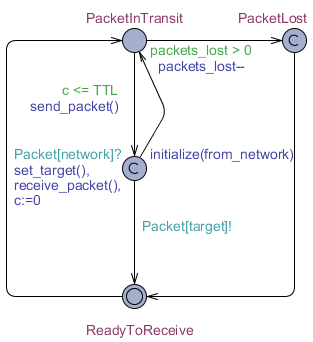
\includegraphics[width=\linewidth]{network_model}
	\end{center}
	\caption{The model of a network}
	\label{fig:figure1}
\end{figure}


\subsubsection{Abstraction from real networks}
\begin{itemize}
\item Our networks have a maximum amount of packets that can be dropped in total for each network automata. This was needed in order to reduce state space to be able to check the model. Also, cases where all packets are dropped are not interesting for us, because that is a case where no connection can be established, and is therefore trivial.
\item Real life networks can handle a large amount of packets in transit simultaneously. But since every instance of the network automata can only handle a single packet at a time, we need one instance for each simultaneous network. With 4 networks hosts can have 1 or more outstanding packets, and is therefore enough to model all cases that are interesting for us.
\end{itemize}


\subsection{Modelling the hosts}
Every host in our model has it's own instance of a host automaton. At the initialization, a local address for the host is set, and an address for the target host, that we want to communicate to. Also, the first step a host needs to make is to assign an initial sequence number it will use.
By using the following transition select statement:
\begin{verbatim}i:SEQ
\end{verbatim}
Where SEQ is defined as 
\begin{verbatim}const int MAX_SEQ = 3;
typedef int[0,MAX_SEQ] SEQ;
\end{verbatim}
We ensure that every possible initial sequence number can be used for checking the model.

Visually, our model has the same layout as the diagram on page 23 of Rfc793. This helps to see how our model maps to the real specification. (See figure \ref{fig:figure2} for our model)
\begin{figure*}
  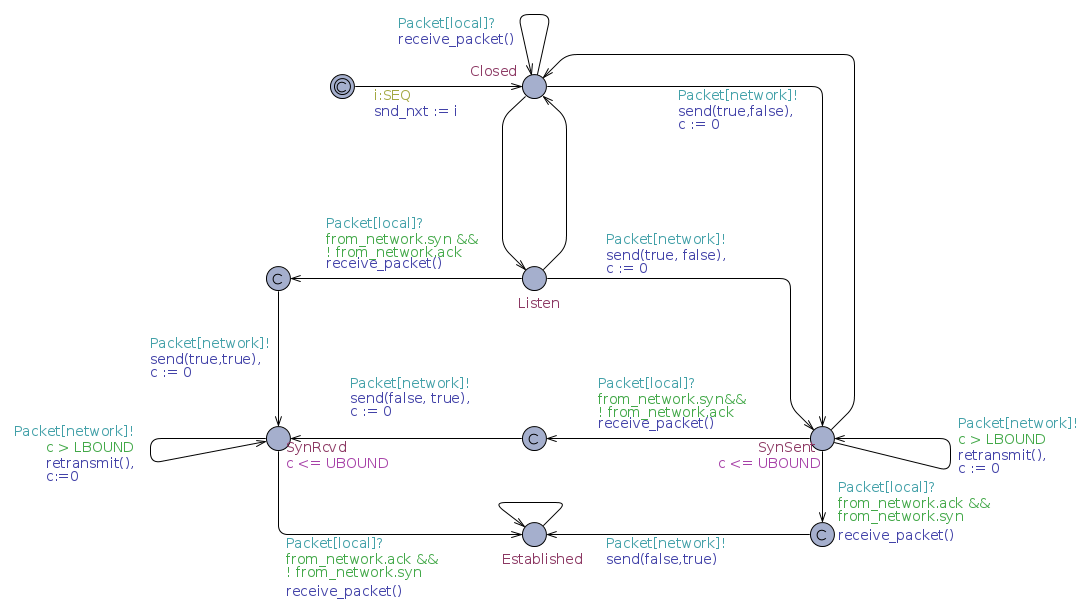
\includegraphics[scale=0.55]{host_model} % at textwidth, the figure takes an entire page
  \caption{The model of a host}
  \label{fig:figure2}
\end{figure*}
We model every state connected to the TCP handshake, namely Closed, Listen, SynSent, RynRcvd and Established. Since we can not synchronize two channels at once, we added committed states between Listen-SynRcvd, SynSent-Established, and SynSent-RynRcvd. This way we can model the behavior of receiving, and then sending a packet as a single action.

Hosts also support a re-send timer if an acknowledgment is not received faster then the round-trip time. This upper bound is not specified in Rfc793, but they suggest that one second is a reasonable value for this. Therefore our UBOUND is set to 600, corresponding to 60,0 seconds. This re-send timer is reset every time a packet is send to the network.

The hosts also check for faulty packets, and discard them. These are the loops at Listen, SynRcvd and SynSent. 

Our hosts are modeled to update all necessary values for sending the next packet when a packet is received. This is defined in our receive packet function:
\begin{verbatim}
bool receive_packet(){
	if (from_network.syn) {
		rcv_nxt = from_network.seqNr;
	}
	if (rcv_nxt == from_network.seqNr) {
		received := from_network;
		if(received.ack){
			snd_nxt = received.ackNr;
		}
		snd_ack = (received.seqNr + 1 + seg_len)%MAX_SEQ;
		rcv_nxt = snd_ack;
		initialize(from_network);
		return true;
	}
	return false;
}
\end{verbatim}

This function handles the receiving of a packet, and returns whether this packet should be accepted, or not.

If the syn flag of the incoming packet is set, the next expected sequence number is initiated . If this is not the case, then the sequence number of the packet is checked against the expected next sequence number.

When a packet is accepted, then the ack that this host will send is set to the received sequence number + 1, modulo the max number of sequence numbers.


\subsubsection{Abstraction from real hosts}
\begin{itemize}
\item The space of sequence numbers is much larger in real hosts, and sequence number wrapping can only occur on very fast networks. But because we do not model real data transmission in the established state, and only focus on the connection set-up, a few sequence numbers are enough to model all interesting cases. Therefore we set our max sequence number to 3.
\item We do not model the behaviour of connection-reset packets that can be send when a host refuses a connection. These reset packets should be used instead of just discarding faulty packets.
\item For real TCP connections, there are many more checks to be done for checking whether a packet will be accepted or not. Also, the expected next sequence number will not always be the last sequence number +1. But since we only model the connection set-up behavior, our simplifications will suffice. Since this behavior matches that particular part of Rfc793.
\item Our model will indefinitely try to re-send a packet if it is not received. This does not match real-world behavior, but since we modeled our networks to only drop a maximum number of packets, this will not matter.
\end{itemize}






\section{Model checking and verification} % (fold)
\label{sec:model_checking_and_verification}
	Because we used Uppaal as our modeling tool, it provides us with an powerful query language to use for verifying our model against the specifications given in Rfc793. Most of these specifications have been discussed in the modeling itself. It would take too long to verify every detail of the model and every model will differ in some way as every model is prone to the creativity of it's designer. We can however guarantee some basic functionalities using the query language. Given that the model is correct, we can test various aspects of the model to check if there are loopholes within the protocol that haven't been uncovered. If there aren't any loopholes, then we can assume that the protocol, given our abstractions as described earlier, is proven correct because all possible states have been explored.
	\subsection{Model Verification} % (fold)
	\label{sub:model_verification}
		As discussed before we want to verify that the model has the basic functionality as described in the request for comments. The first thing that should be guaranteed is that two hosts can connect to each other. This is easily verified by the following query stating that there is a state such that both Host1 and Host2 are in the Established state:
		\begin{verbatim}
			E<> Host1.Established 
			and Host2.Established
		\end{verbatim}
		This is verified. Because this holds, we know that the hosts can be connected since this is defined as both hosts being in the Established state.

		Furthermore one host shouldn't be in the established state, thinking there is a connection, while the the other host is still in the Listen, Closed or SynSent state, knowing nothing about an connection whatsoever. This can be verified using the following query:
		\begin{verbatim}
			A[] not ((Host1.Closed or Host1.Listen 
or Host1.SynSent) and Host2.Established)
		\end{verbatim}
		This query states that there is not a state were Host1 is in the Closed, Listen or SynSent state while Host2 is in the Established state. Note that Host1 can be in the SynRcvd state while the other has an established connection. This would mean the first host is waiting for the last packet sent by the second host.

		Finally we want to guarantee that the protocol does not have places were the hosts get stuck and can not progress to a new state. This phenomenon is a deadlock in this model, where there is a state where no any options to advance are available. To test this we need to make sure that our established state transitions back to itself, so it does not result in an deadlock. Then we can check for deadlocks using the simple query:
		\begin{verbatim}
			A[] not deadlock
		\end{verbatim}

		Our model passes these queries as is shown in figure \ref{fig:verifier}, proving that an implementation following this model has basic functionality.
		\begin{figure}[h!]
			\begin{center}
				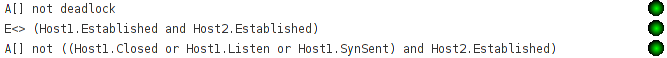
\includegraphics[width=\linewidth]{verifier.png}
			\end{center}
			\caption{Uppaal verifier - basic queries}
			\label{fig:verifier}
		\end{figure}
	% subsection model_verification (end)
	\subsection{Guaranteeing an connection} % (fold)
	\label{sub:guaranteeing_an_connection}
		The queries become more interesting when trying to analyse a specific aspect of the model. The aspect we are interested in, is a guaranteed connection set-up. This means that when both hosts are able to set-up a connection and both hosts want a connection, the connection will always set-up. Hosts are only able to set-up a connection when they are not in the Init or Closed state. To force the hosts to enter the other states we remove the transition from the Closed state back to itself and guarantee the host leaves the Closed state by making it an committed state. To make sure a hosts does not deny the connection set-up we remove the possibility for hosts to return to the closed state. With these changes to the model we can now write a query that checks if the model does guarantee a connection between the two hosts given that they both try or accept connection set-up.

		\subsubsection{Case 1: Basic three-way handshake}
		First we prove that if the connection is not set-up using an simultaneous initiation, that there will always follow an connection between the two hosts. To check if this condition holds within our model we need to disable the possibility for the simultaneous initiation. We do this by removing the transition from the Listen state to the SynSent state and forcing within the query that one host visits the SynSent state, while the other visits the Listen state. To check if these conditions result in an established connection we use the following query:
		\begin{verbatim}
			(Host1.Listen and Host2.SynSent) -->
			(Host1.Established and Host2.Established)
		\end{verbatim}
		This query holds in our model as is shown in figure \ref{fig:verifier2}.
		\begin{figure}[h!]
			\begin{center}
				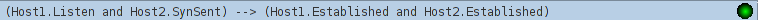
\includegraphics[width=\linewidth]{verifier-listen.png}
			\end{center}
			\caption{Uppaal verifier - Basic Three-way Handshake}
			\label{fig:verifier2}
		\end{figure}
		% subsubsection Case 1: Basic three-way handshake (end)
		
		\subsubsection{Case 2: Simultaneous connection request}
		Now we prove that when a simultaneous connection request happens, there will always be a established connection between both hosts. To check for this condition, we remove the transition between Closed and Listen. This way, both hosts have to establish a connection using a simultaneous connection set-up. Within the query we force that both hosts pass the SynSent state. Again, we had to remove the packet discarding in the closed state. This is due to the fact that we do not handle reset packets. Please see the next section for a related problem.
		\begin{verbatim}
			(Host1.SynSent and Host2.SynSent) -->
			(Host1.Established and Host2.Established)
		\end{verbatim}
		This query holds in our model as is shown in figure \ref{fig:verifier3}.
		\begin{figure}[h!]
			\begin{center}
				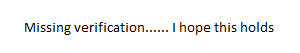
\includegraphics[width=\linewidth]{verifier-simul.png}
			\end{center}
			\caption{Uppaal verifier - Simultaneous Connection Request}
			\label{fig:verifier3}
		\end{figure}
		
		% subsubsection Case 2: Simultaneous connection request (end)
		\subsubsection{Issues concerning the checking of this model}
		At the moment it is not possible to check both queries in the same model without removing some connections. This is due to the fact that we do not model the behaviour of reset-packets. Because connection cannot be actively reset, there exists an infinite loop when the following occurs:
		\begin{enumerate}
			\item Host1 sends a Syn packet, and is now in the SynSent state
			\item Host2 was in the Closed state, so the packet gets discarded
			\item Host2 now sends a Syn packet to Host1 before Host1's re-send timer triggered.
			\item Host1 thinks this is a simultaneous connection request and goes into the SynRcvd state. 
			\item Host2 is now waiting for a Syn, or a SynAck packet and keeps re-sending Syn packets.
			\item Host1 is now waiting for a Ack packet, and keeps re-sending Ack packets.
		\end{enumerate}
		They may exist cases where this edge case exists because of interesting timings, even with Reset packages. But this is outside the scope of this project
		% subsubsection Issues concerning the checking of this model (end)
	% subsection guaranteeing_an_connection (end)
% section model_checking_and_verification (end)
	

\section{Conclusions}
		In this report we have proven the correctness of the basic three-way handshake and the simultaneous connection set-up on a simplified model of the TCP handshake. In order to check the model of a more realistic implementation of the TCP protocol, one has to add some missing parts, like the use of reset packets.


\end{document}
